\documentclass[11pt]{article}

\usepackage[margin=1in]{geometry}
\usepackage{graphicx}
\usepackage{booktabs}
\usepackage{hyperref}
\usepackage{float}

\title{Paper 001a: Artifact Atlas for Causal Observer Ladders}
\author{xPRIMEray}
\date{2026-04-21}

\begin{document}

\maketitle

\begin{abstract}
This document is a barebones artifact companion to the causal observer ladder manuscript.
It assembles the generated figures, analysis plots, and supporting references from the approved
wormhole observer ladder baseline without introducing new rendering runs.
The goal is simple curation: keep the figure set visible, citable, and easy to reuse in later drafts.
\end{abstract}

\section{Source Artifact Set}

Primary checkpoint sequence summary:
\begin{quote}
\url{/home/bb/code/godot_xPRIMEray/output/fixture_runs/fixture_011_wormhole_checkpoint_sequence/2026-04-20T22-26-39/checkpoint_sequence_summary.json}
\end{quote}

Primary manuscript:
\begin{quote}
\url{/home/bb/code/godot_xPRIMEray/Docs/papers/paper_001_causal_observer_ladders/paper.md}
\end{quote}

\section{Core Ladder Figures}

\begin{figure}[H]
  \centering
  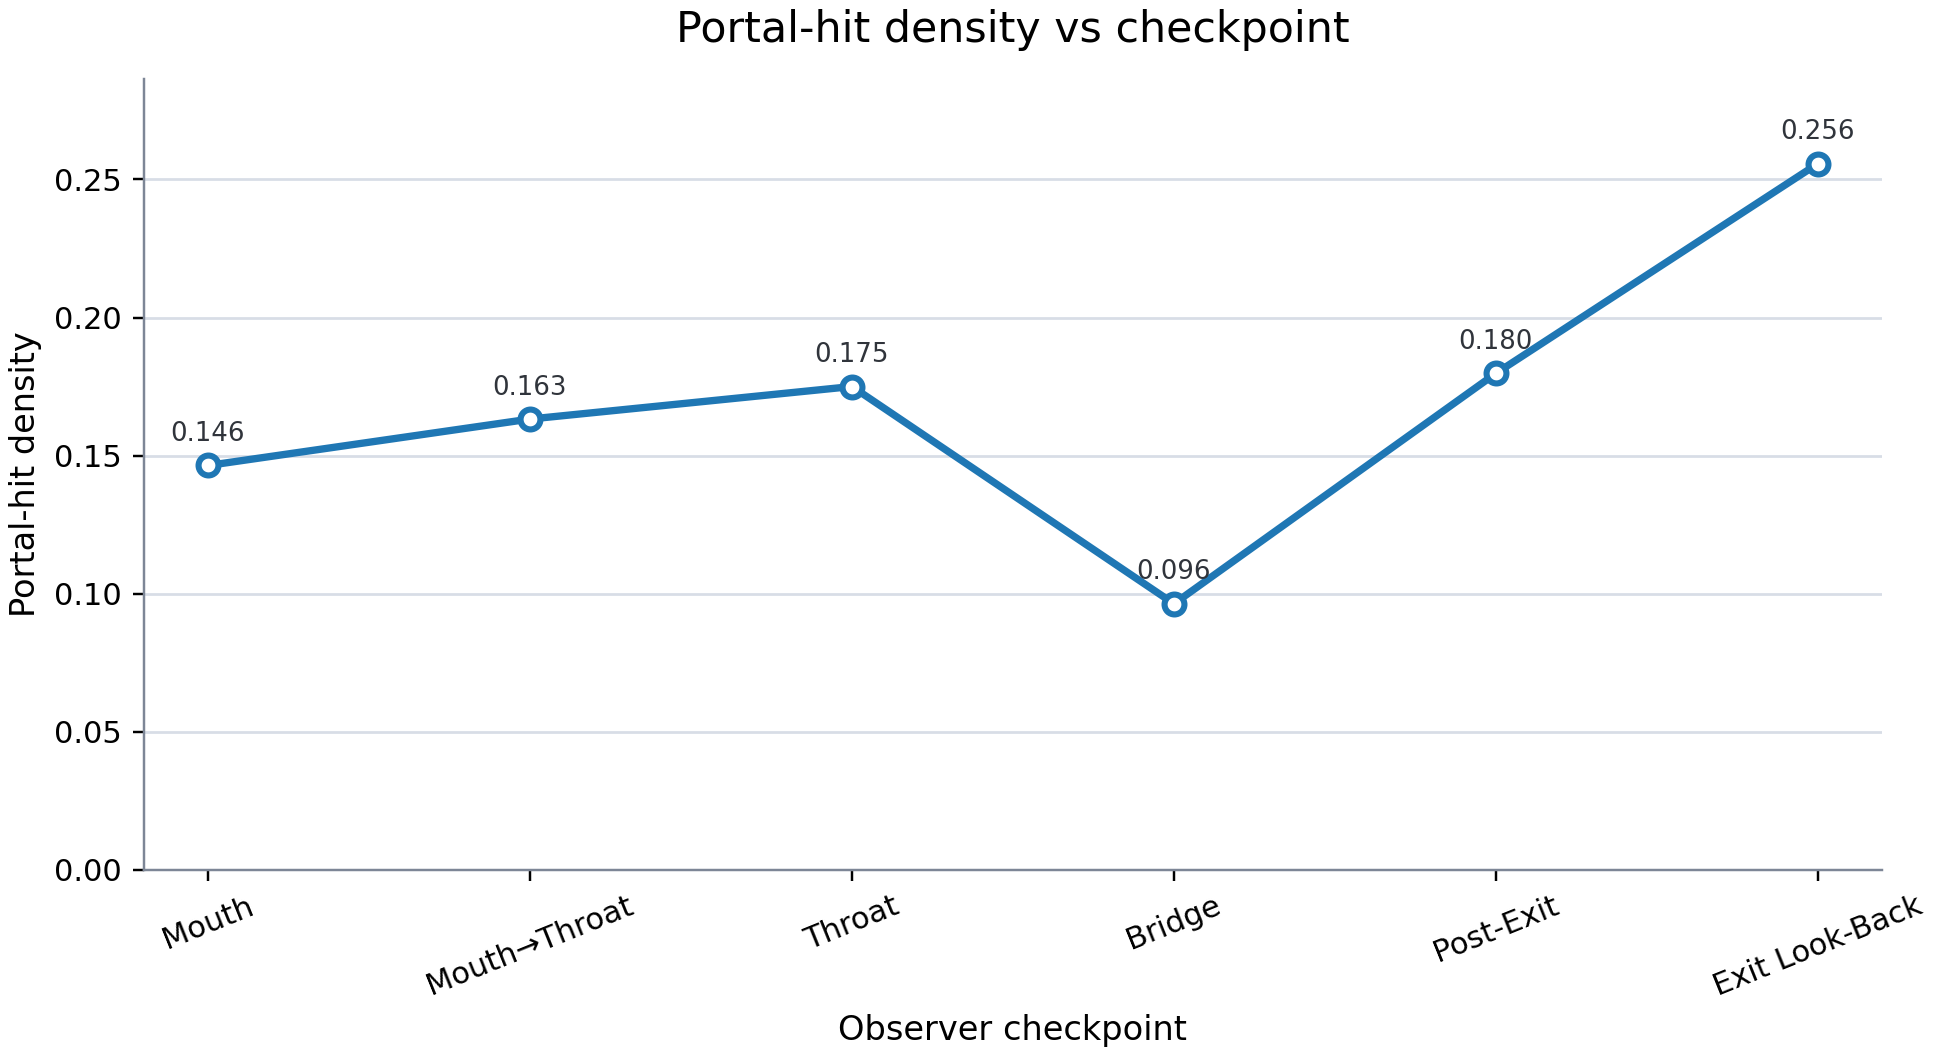
\includegraphics[width=0.82\textwidth]{../../paper_001_causal_observer_ladders/figures/portal_hit_density_vs_checkpoint.png}
  \caption{Portal-hit density across the approved observer ladder.}
\end{figure}

\begin{figure}[H]
  \centering
  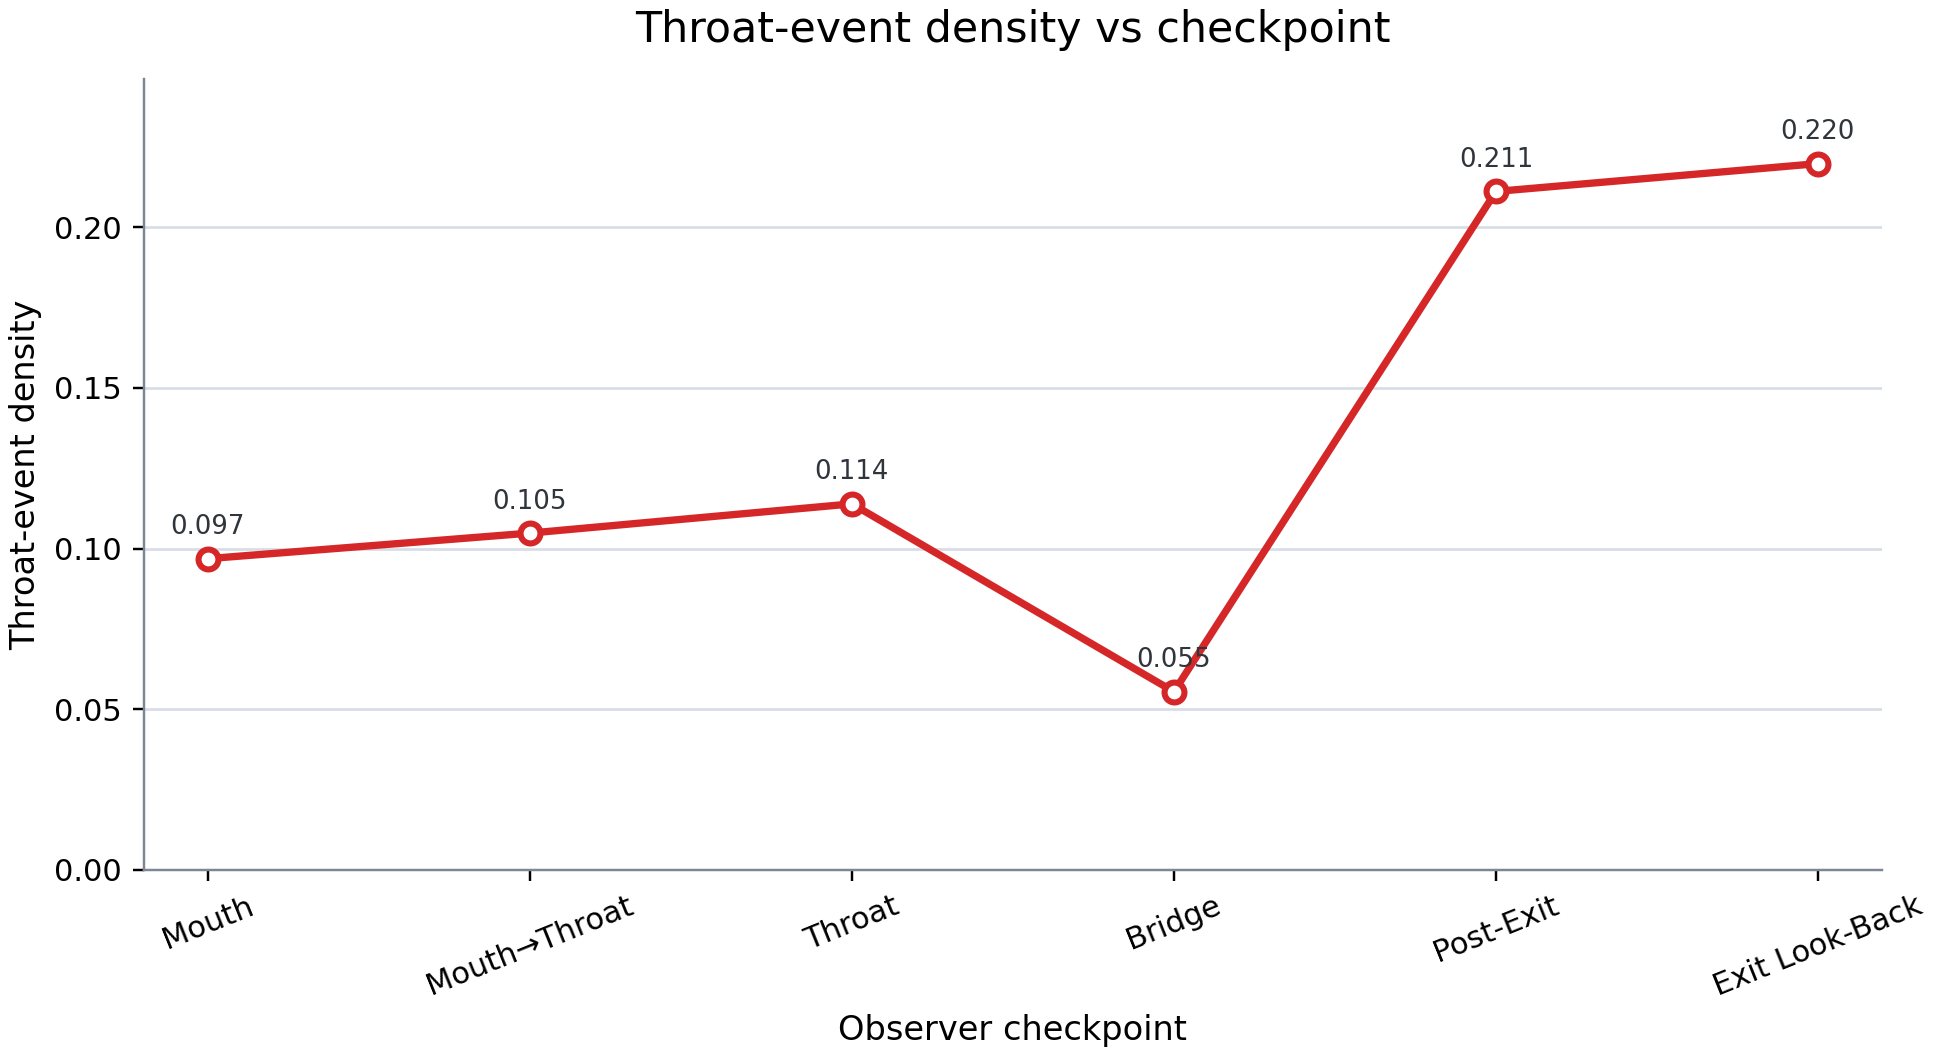
\includegraphics[width=0.82\textwidth]{../../paper_001_causal_observer_ladders/figures/throat_event_density_vs_checkpoint.png}
  \caption{Throat-event density across the approved observer ladder.}
\end{figure}

\begin{figure}[H]
  \centering
  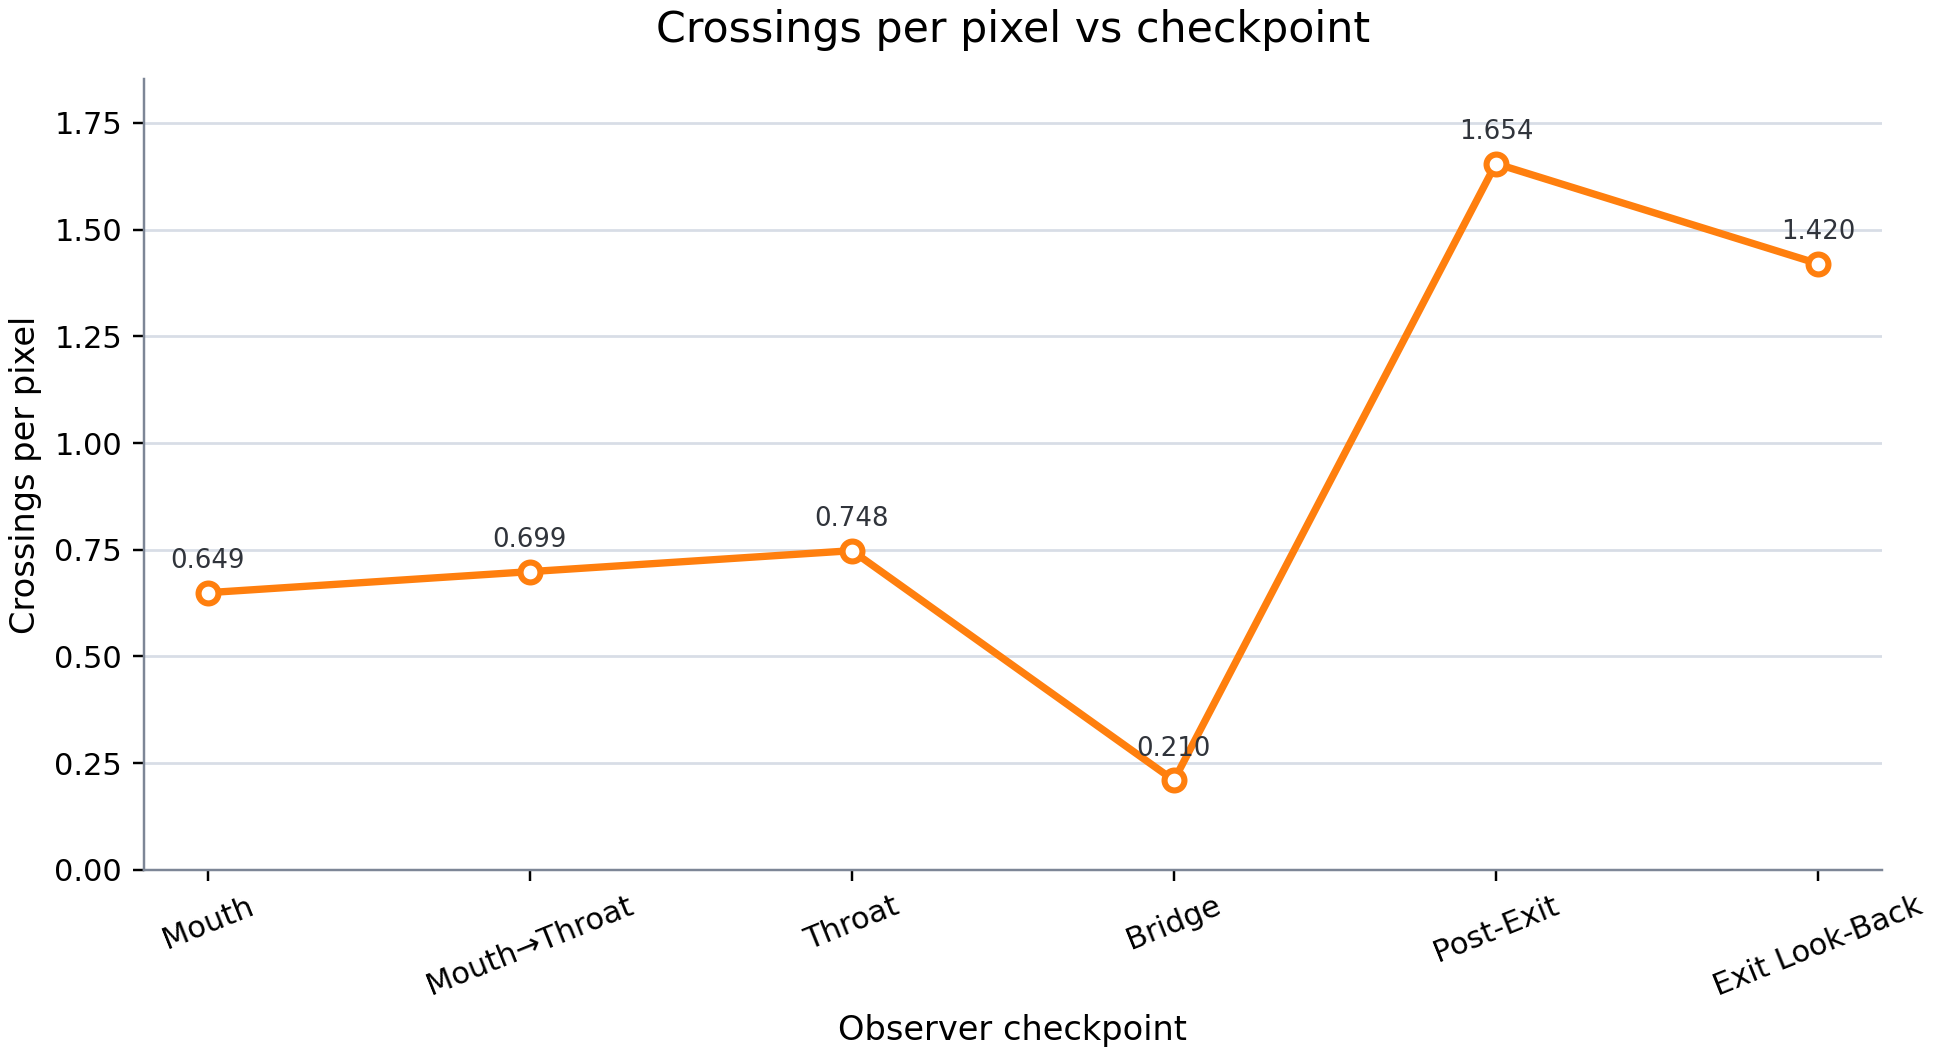
\includegraphics[width=0.82\textwidth]{../../paper_001_causal_observer_ladders/figures/crossings_per_pixel_vs_checkpoint.png}
  \caption{Crossings per pixel across the approved observer ladder.}
\end{figure}

\begin{figure}[H]
  \centering
  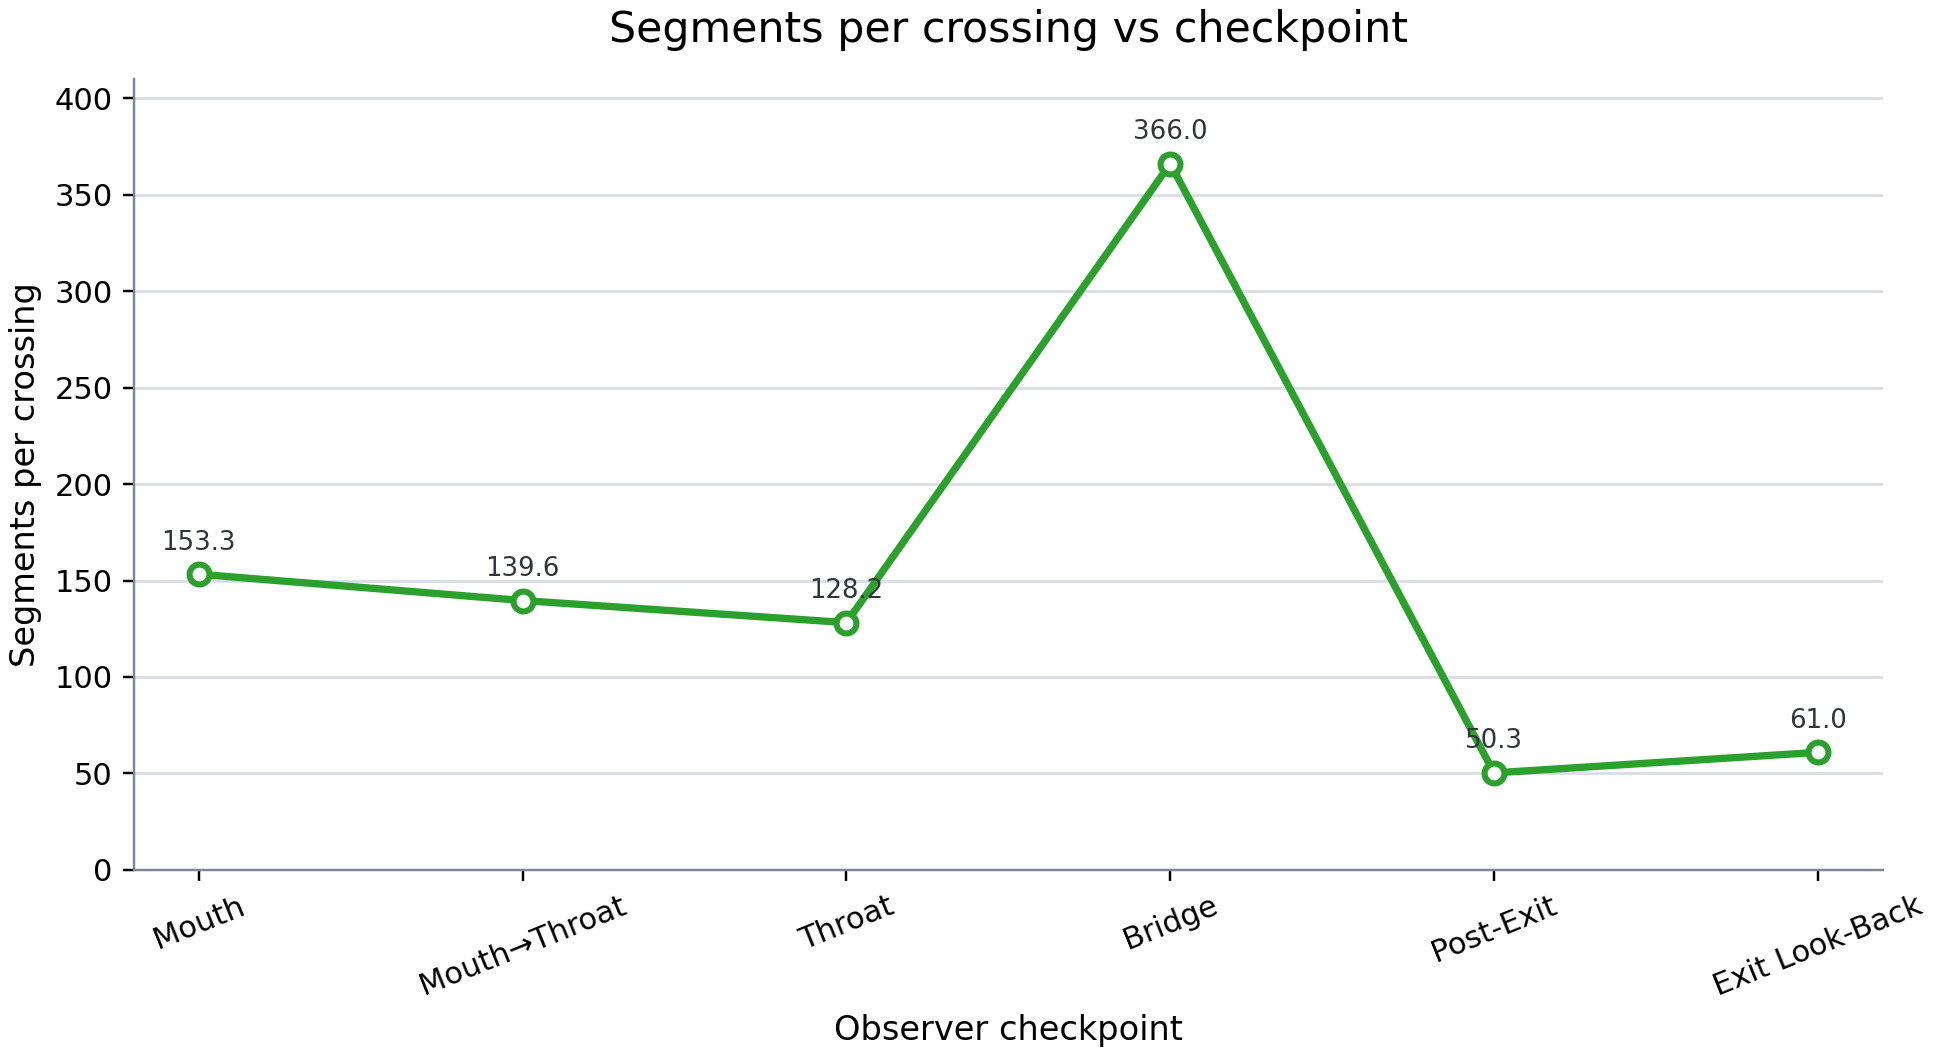
\includegraphics[width=0.82\textwidth]{../../paper_001_causal_observer_ladders/figures/segments_per_crossing_vs_checkpoint.png}
  \caption{Segments per crossing across the approved observer ladder.}
\end{figure}

\begin{figure}[H]
  \centering
  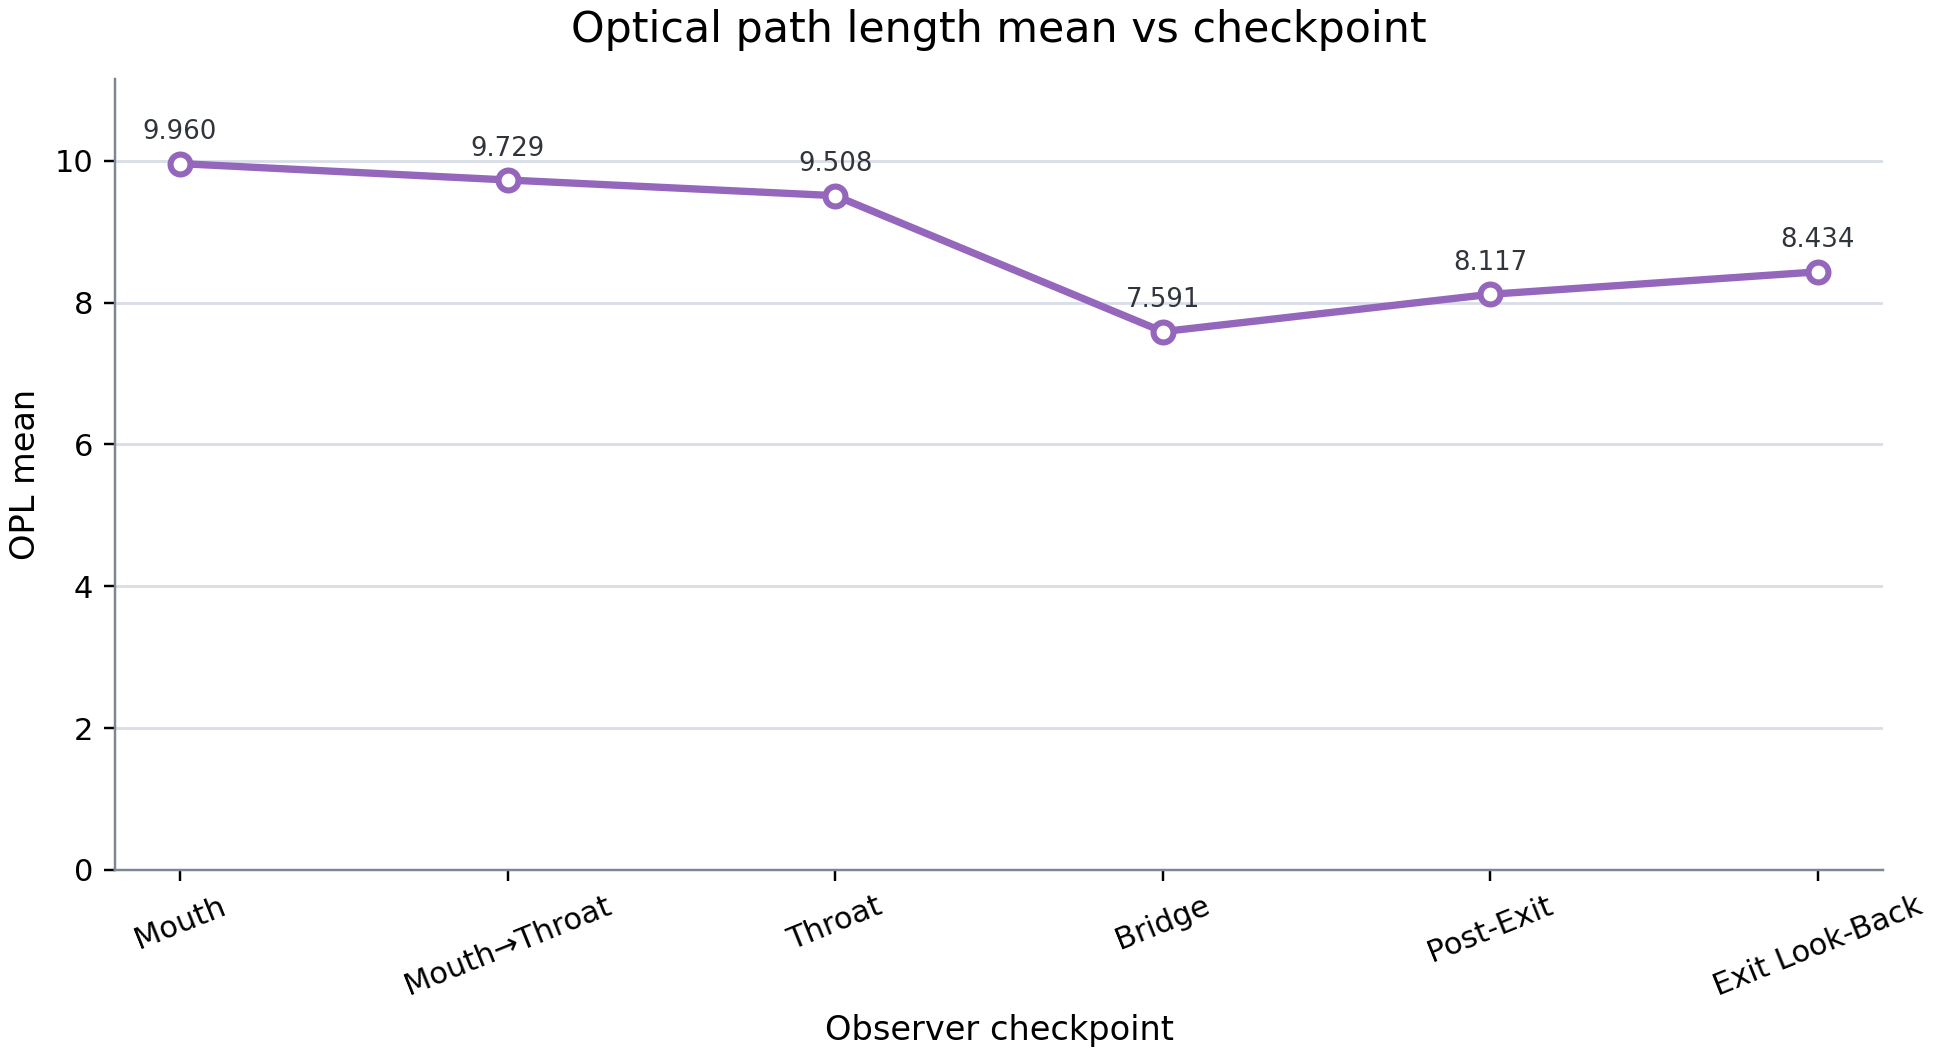
\includegraphics[width=0.82\textwidth]{../../paper_001_causal_observer_ladders/figures/opl_mean_vs_checkpoint.png}
  \caption{Mean optical path length across the approved observer ladder.}
\end{figure}

\section{Cluster and Anomaly Figures}

\begin{figure}[H]
  \centering
  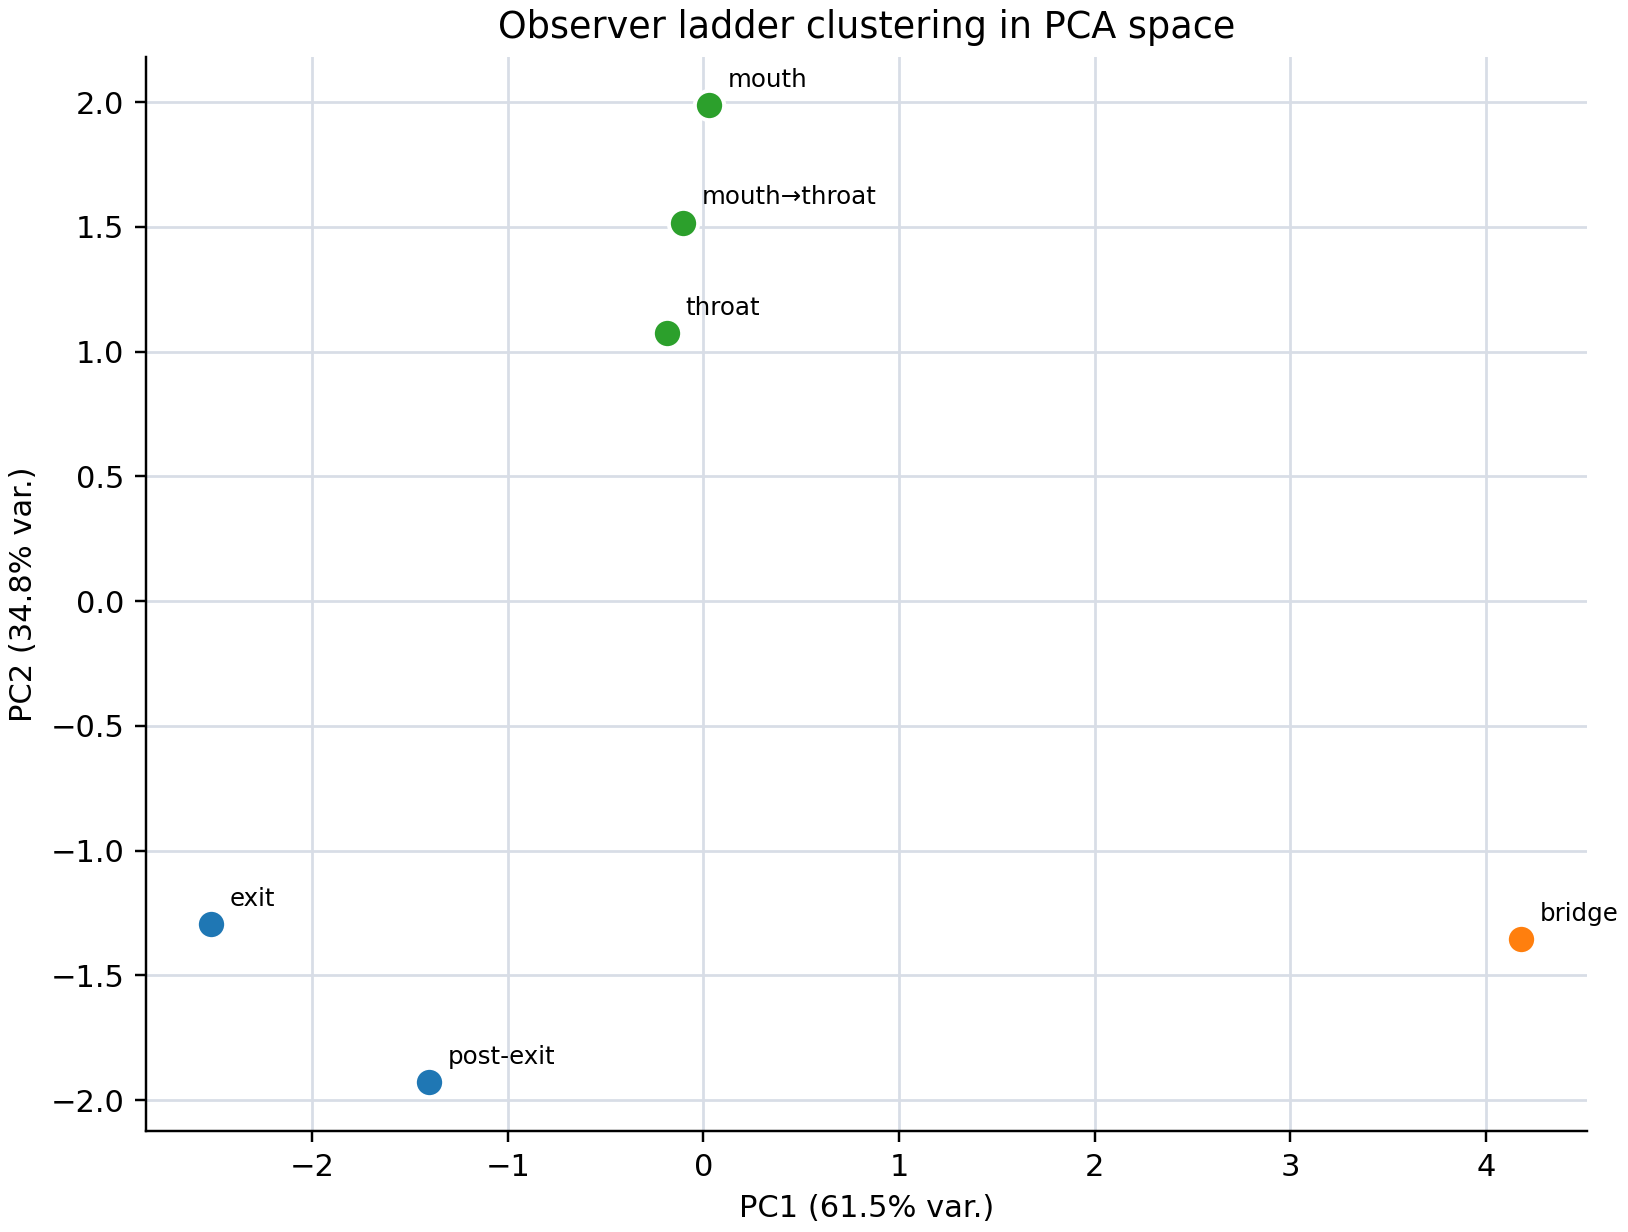
\includegraphics[width=0.82\textwidth]{../../paper_001_causal_observer_ladders/figures/cluster_pca_scatter.png}
  \caption{PCA projection of checkpoint clustering.}
\end{figure}

\begin{figure}[H]
  \centering
  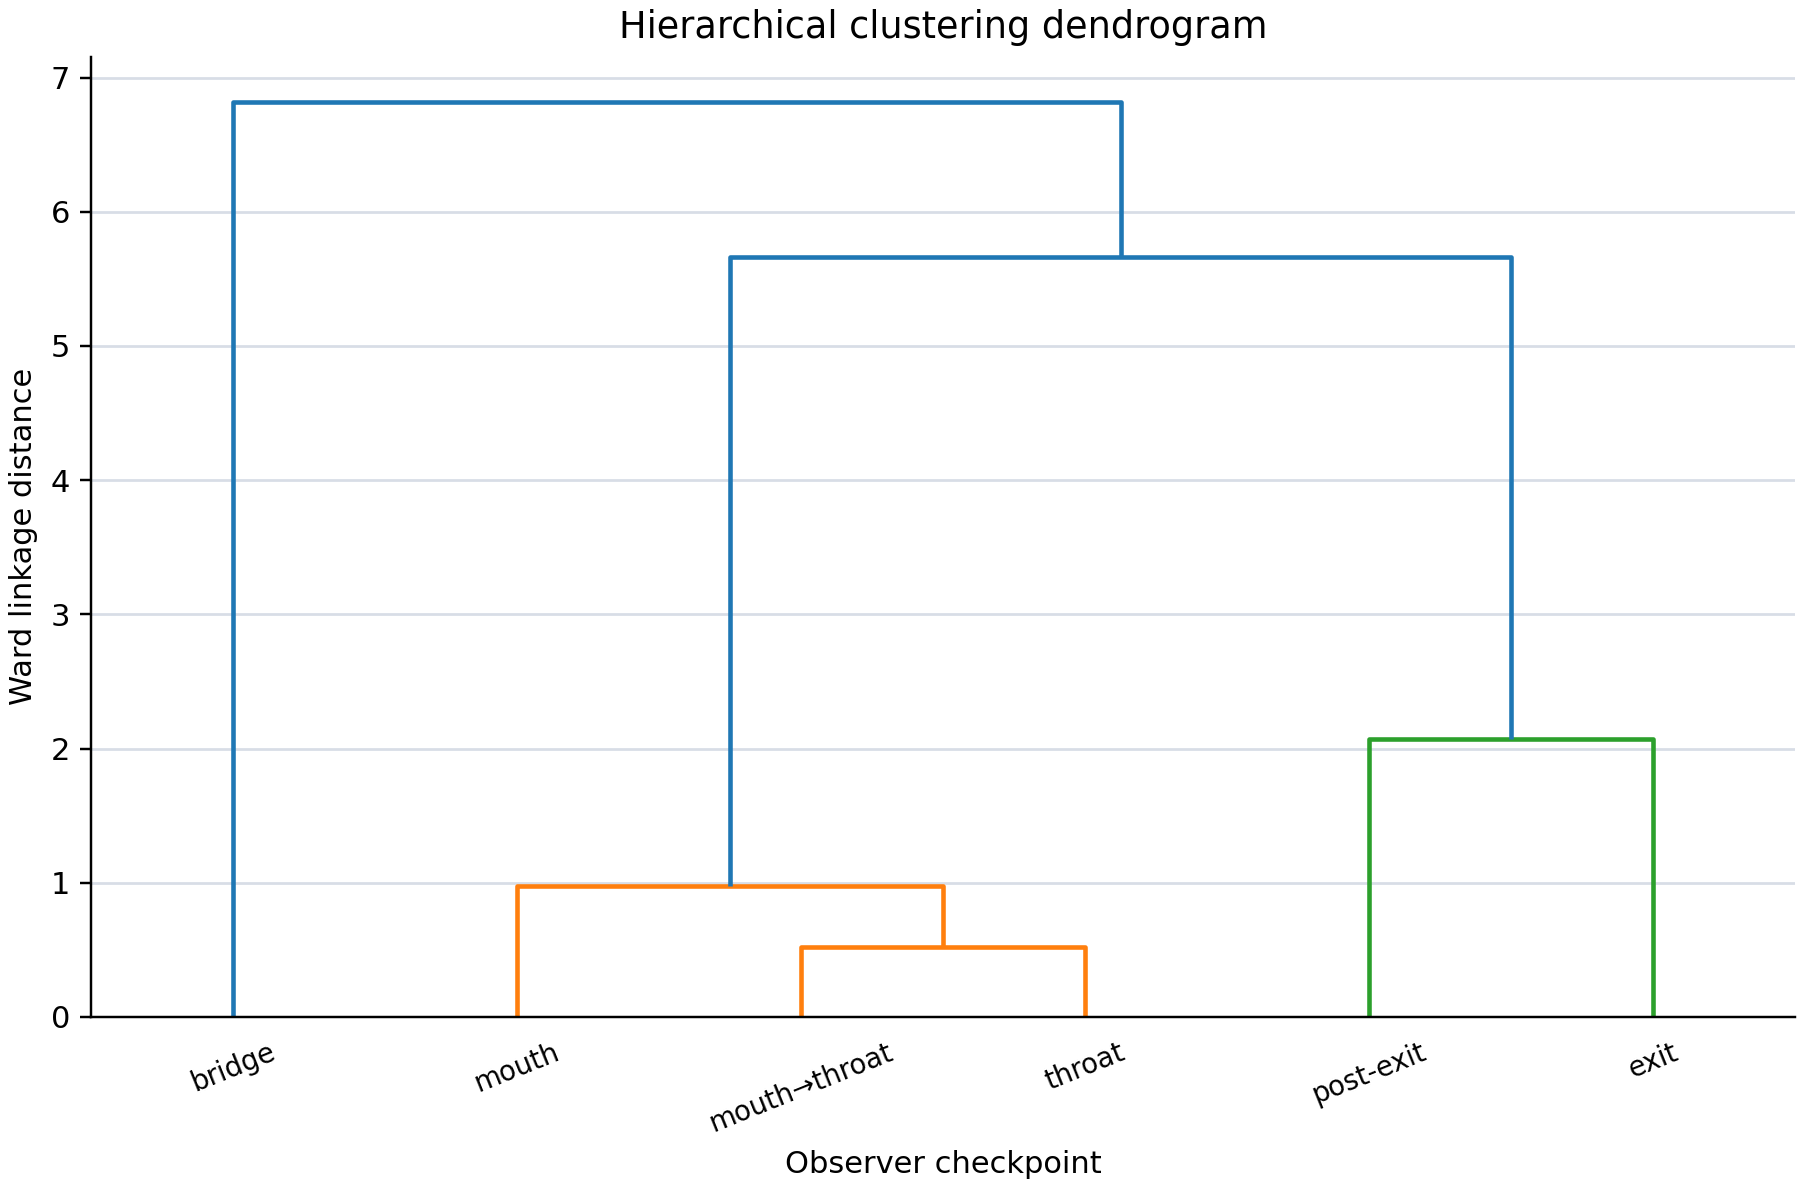
\includegraphics[width=0.82\textwidth]{../../paper_001_causal_observer_ladders/figures/cluster_dendrogram.png}
  \caption{Hierarchical clustering dendrogram for the observer ladder.}
\end{figure}

\begin{figure}[H]
  \centering
  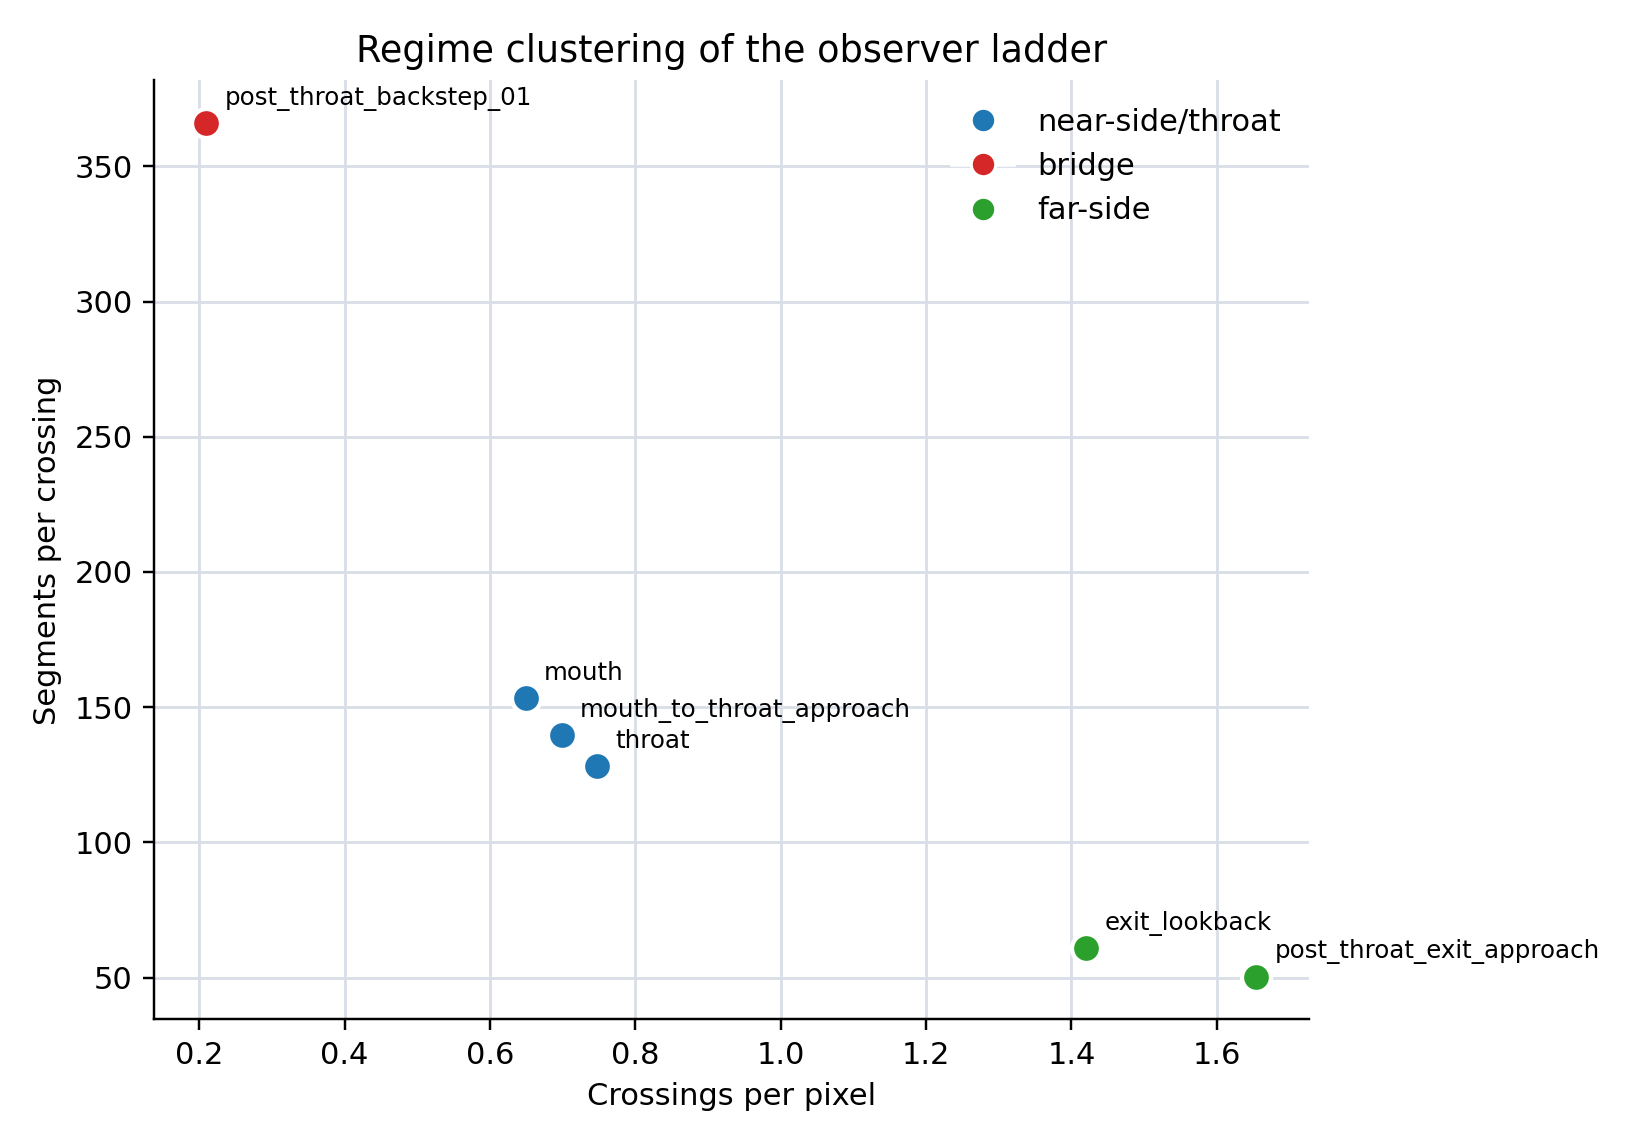
\includegraphics[width=0.82\textwidth]{../../paper_001_causal_observer_ladders/analysis/figures/regime_clustering.png}
  \caption{Artifact-only regime clustering derived from the checkpoint summary.}
\end{figure}

\begin{figure}[H]
  \centering
  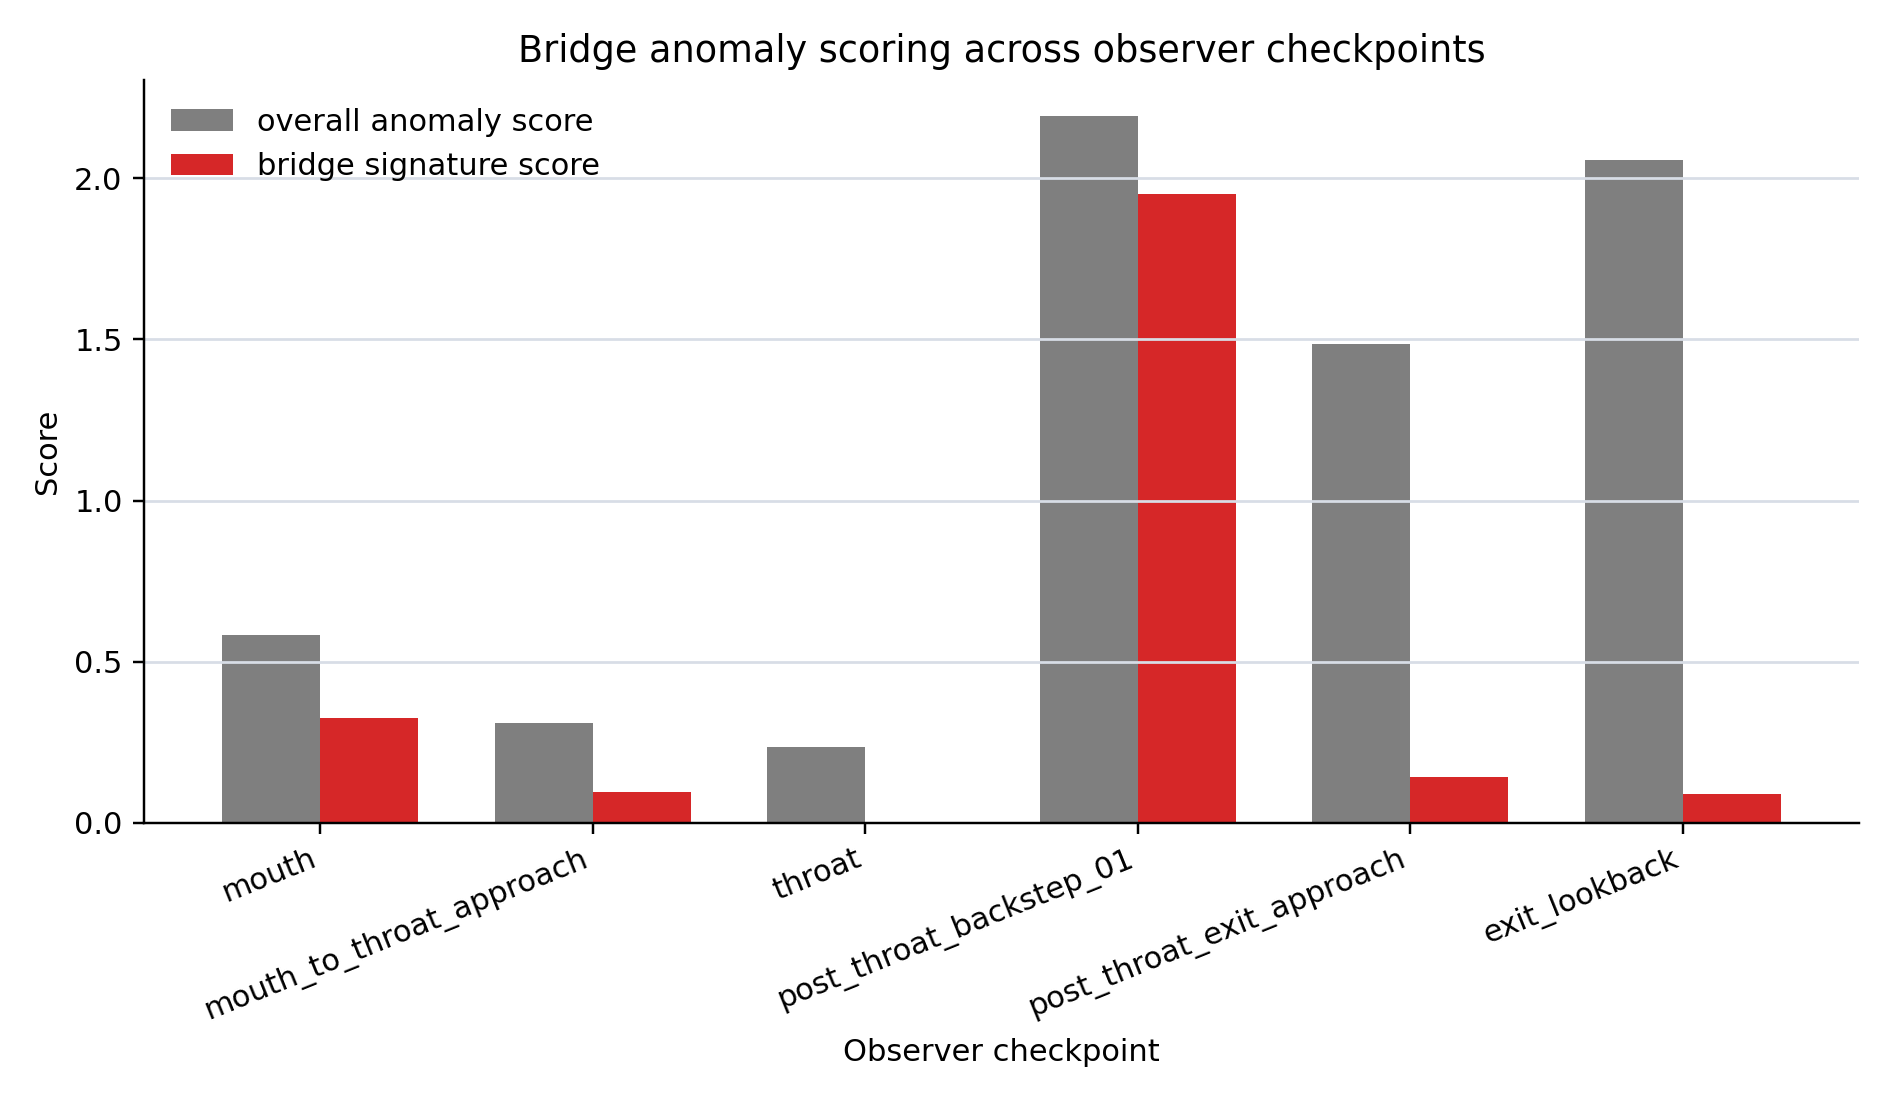
\includegraphics[width=0.82\textwidth]{../../paper_001_causal_observer_ladders/analysis/figures/bridge_anomaly_scores.png}
  \caption{Bridge anomaly scoring from the derived checkpoint metrics.}
\end{figure}

\begin{figure}[H]
  \centering
  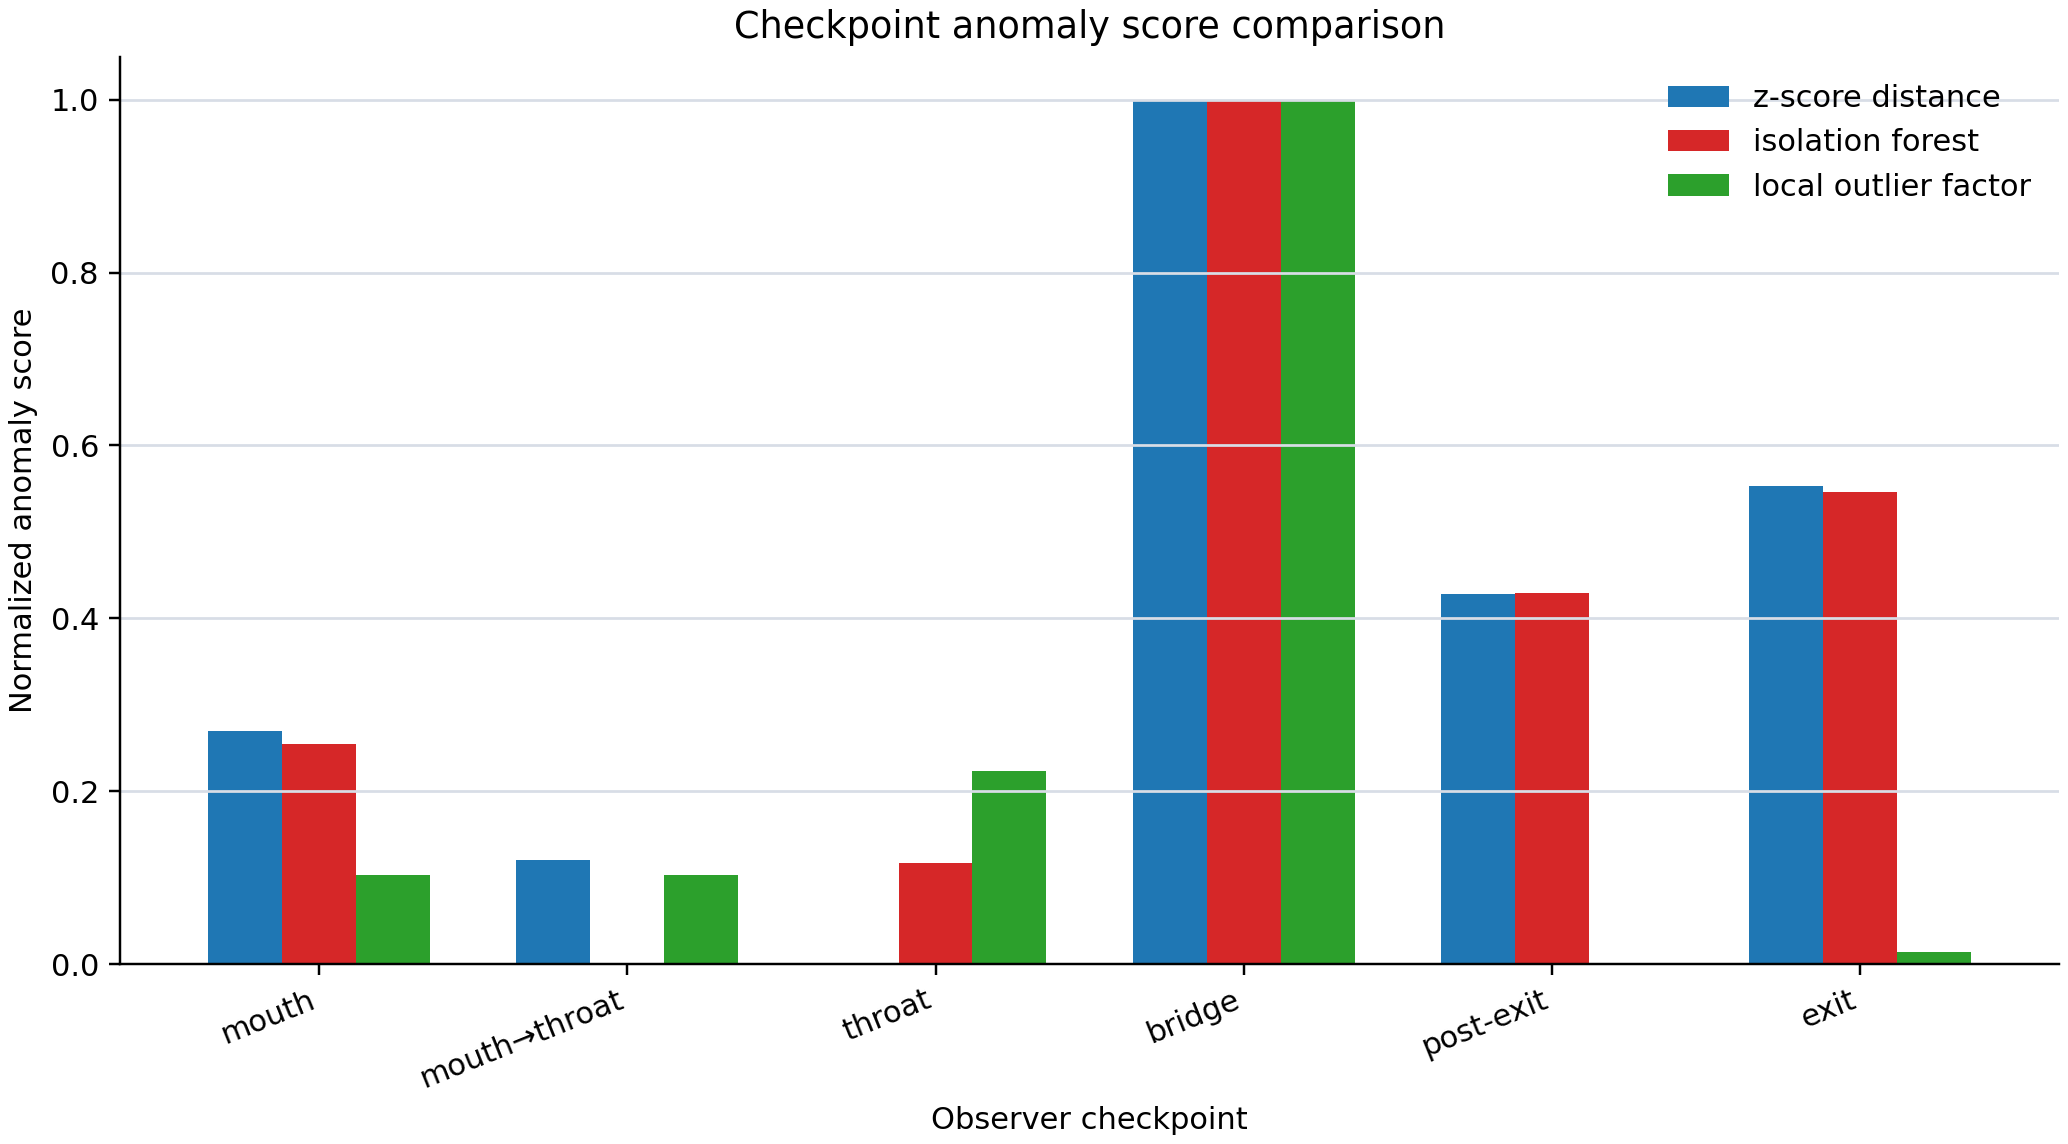
\includegraphics[width=0.82\textwidth]{../../paper_001_causal_observer_ladders/analysis/anomaly_detection/figures/checkpoint_anomaly_scores.png}
  \caption{Multi-method checkpoint anomaly scores.}
\end{figure}

\section{Periodicity and Morphology Figures}

\begin{figure}[H]
  \centering
  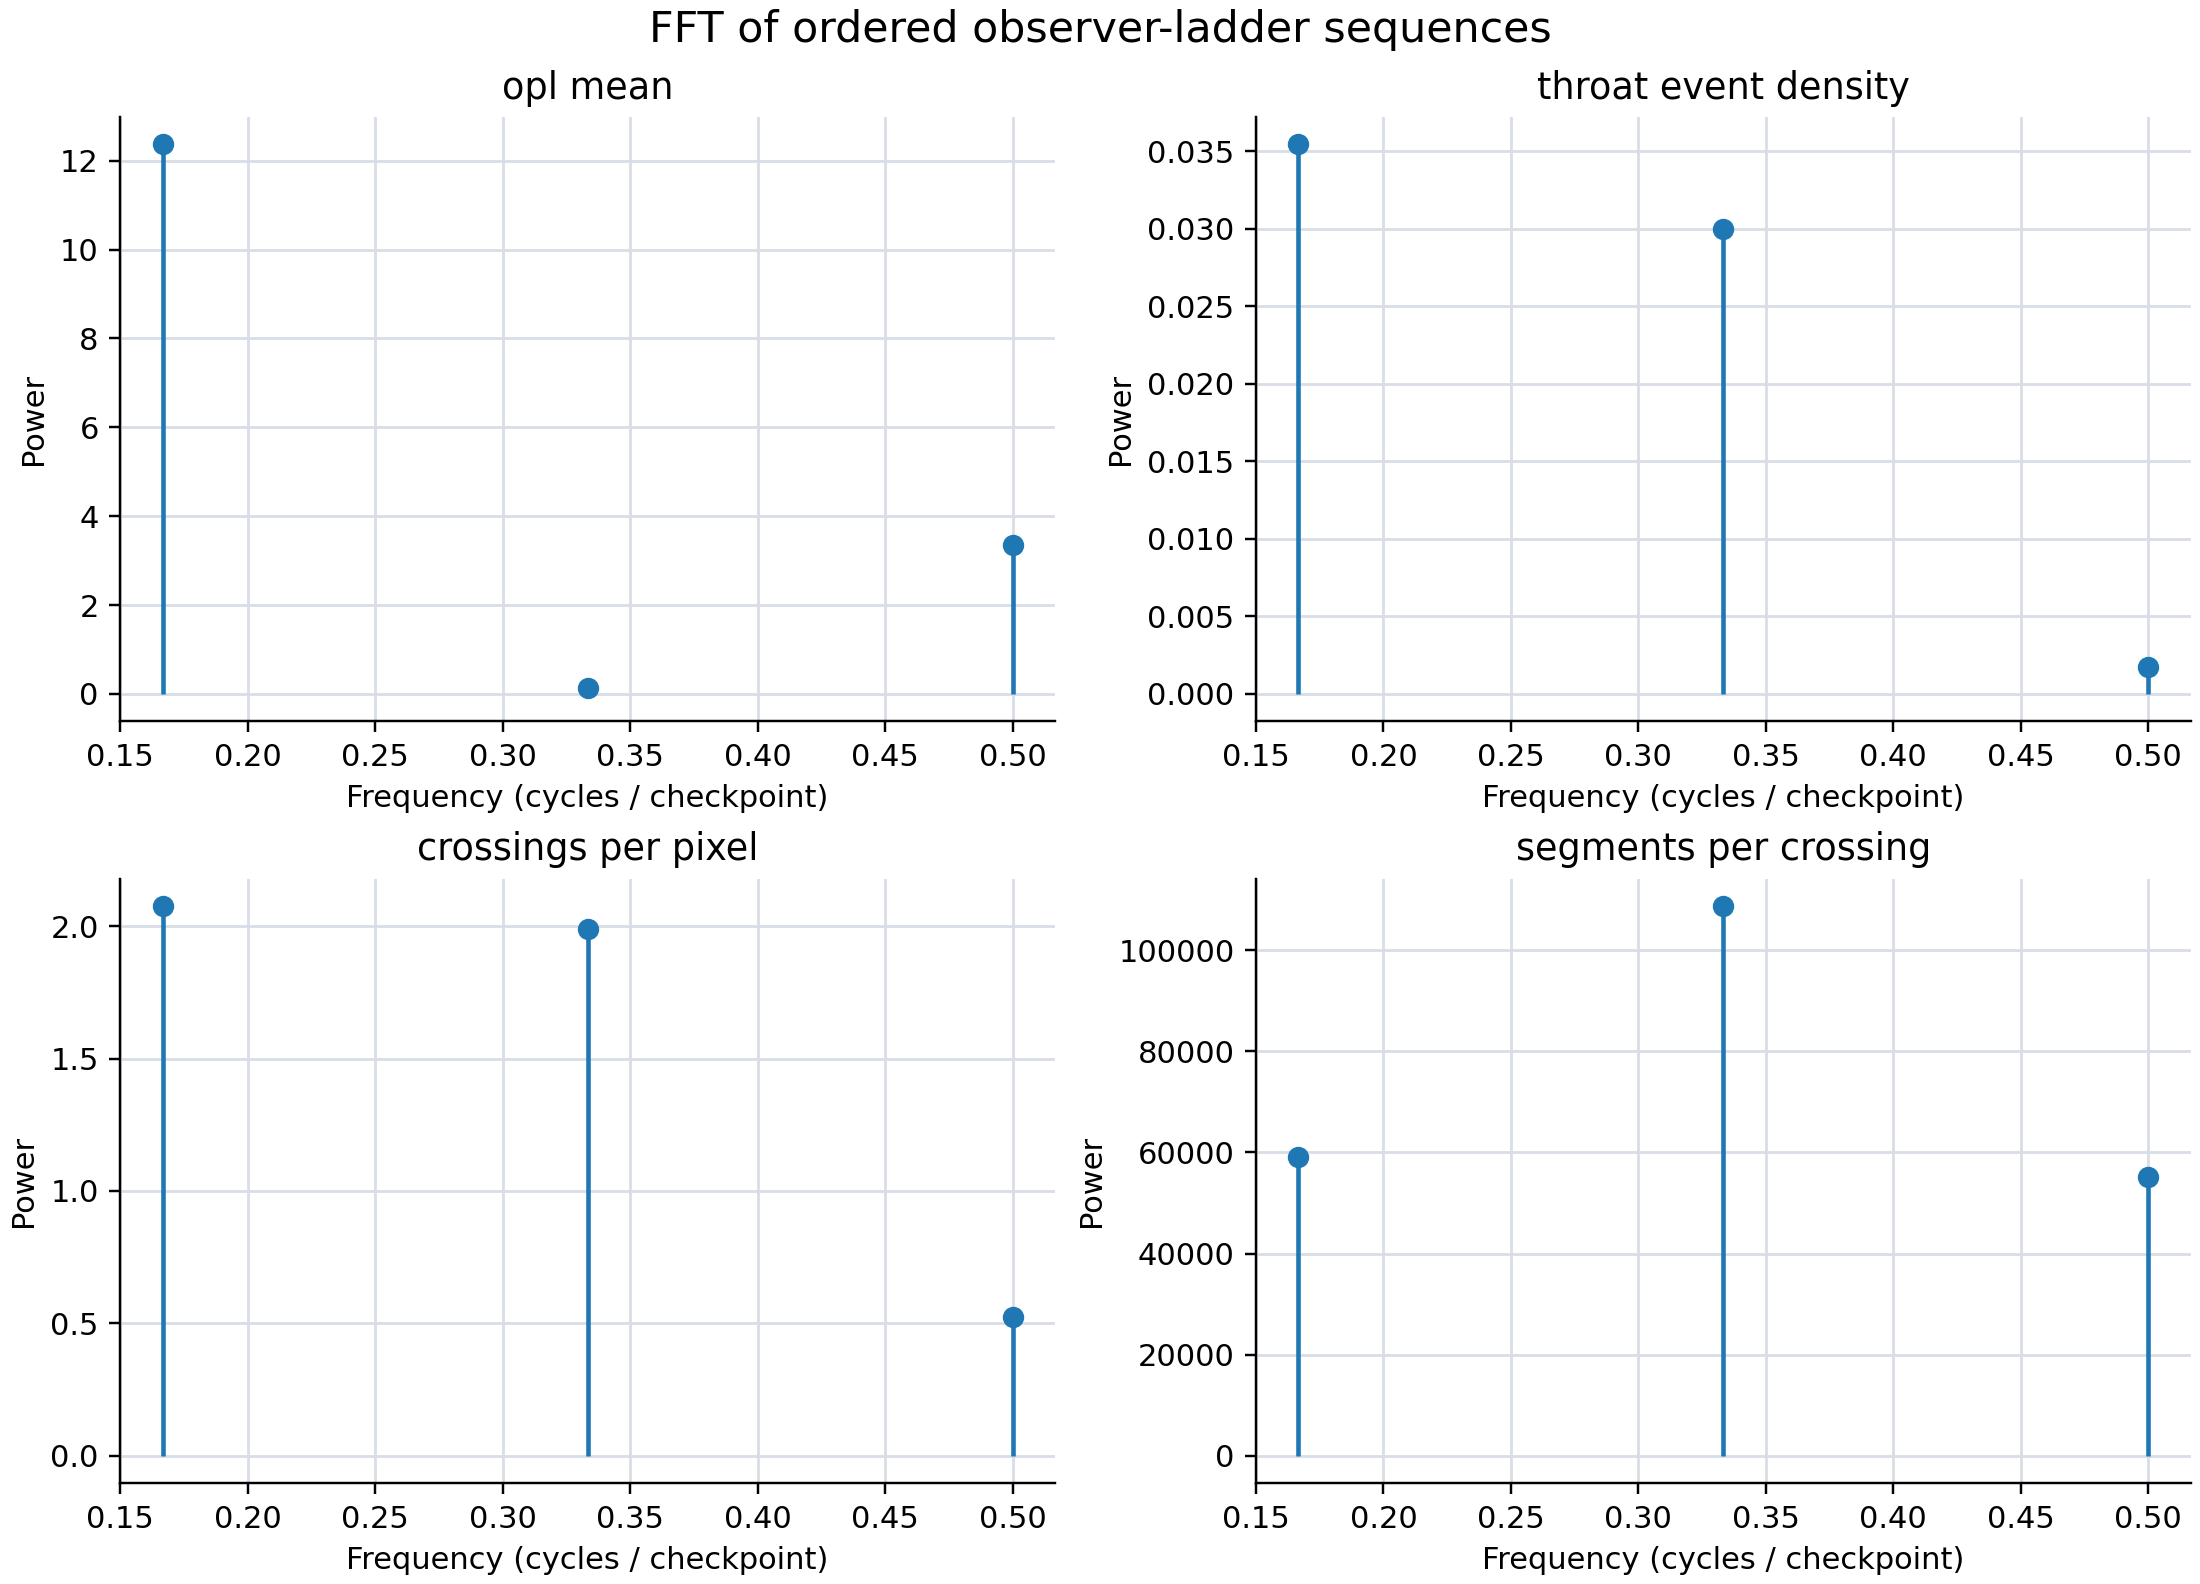
\includegraphics[width=0.82\textwidth]{../../paper_001_causal_observer_ladders/analysis/periodicity/figures/sequence_fft.png}
  \caption{FFT of ordered observer-ladder sequences.}
\end{figure}

\begin{figure}[H]
  \centering
  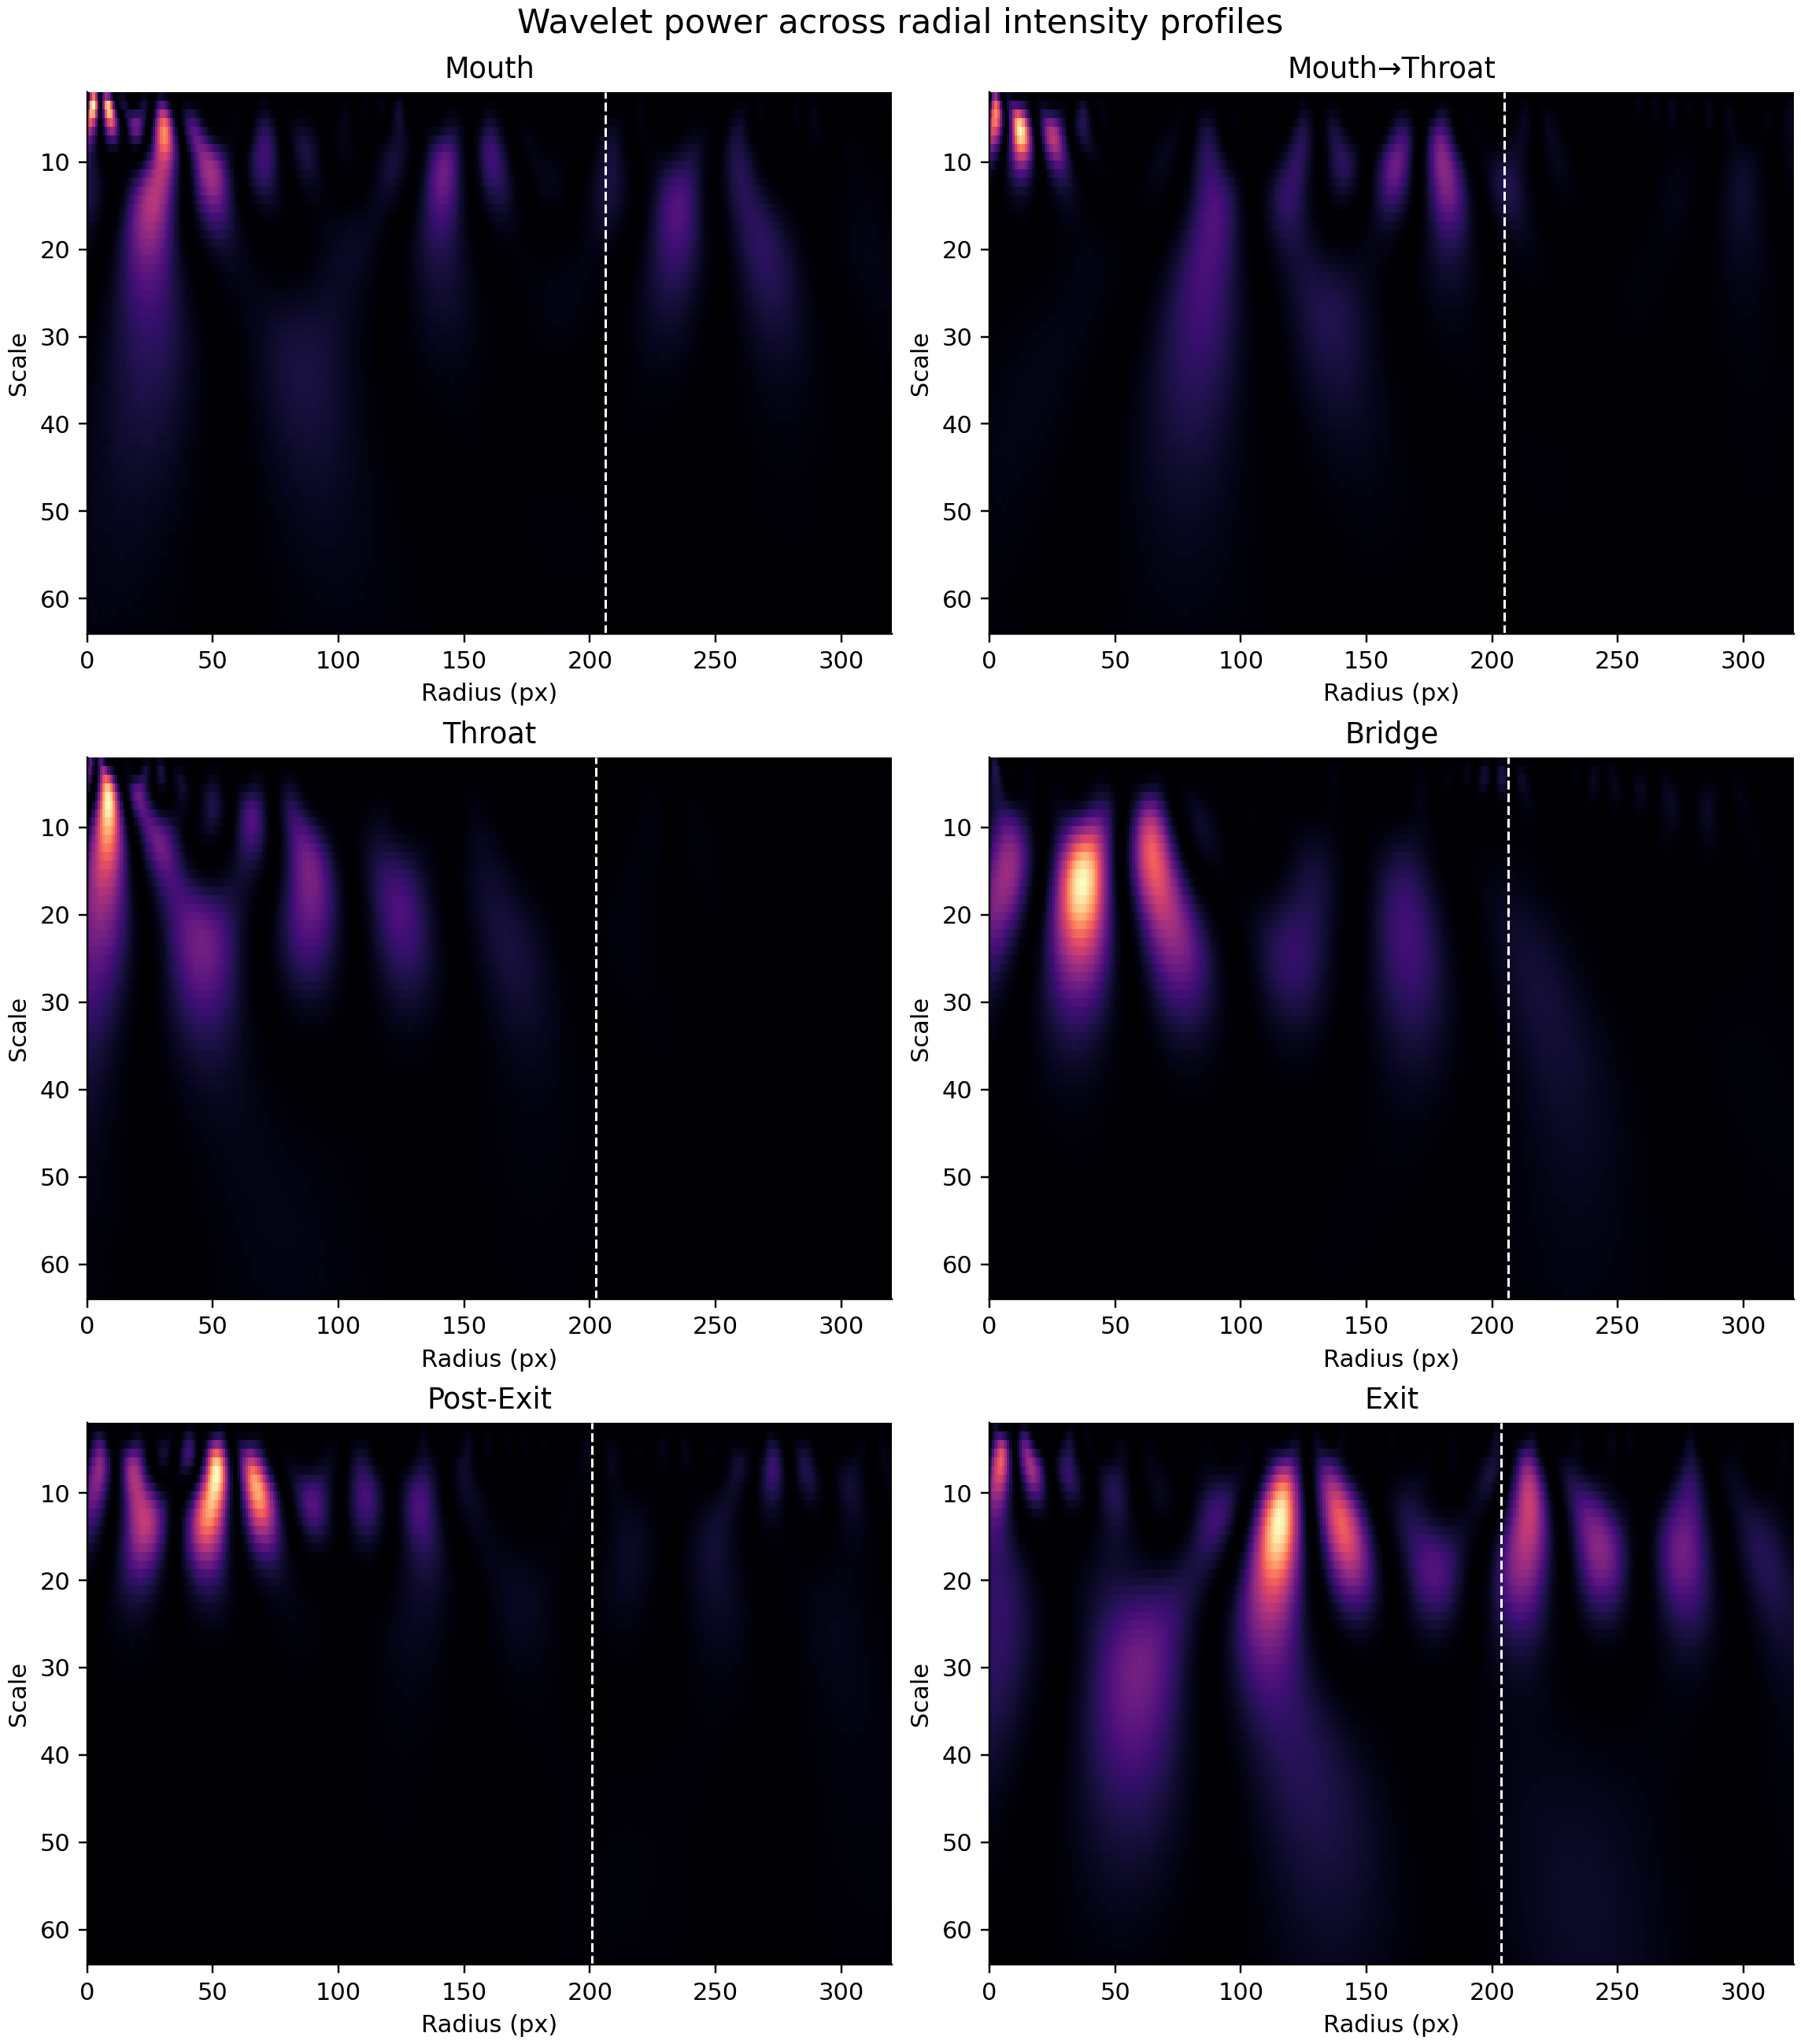
\includegraphics[width=0.82\textwidth]{../../paper_001_causal_observer_ladders/analysis/periodicity/figures/radial_profile_wavelets.png}
  \caption{Wavelet power across radial intensity profiles reconstructed from debug captures.}
\end{figure}

\begin{figure}[H]
  \centering
  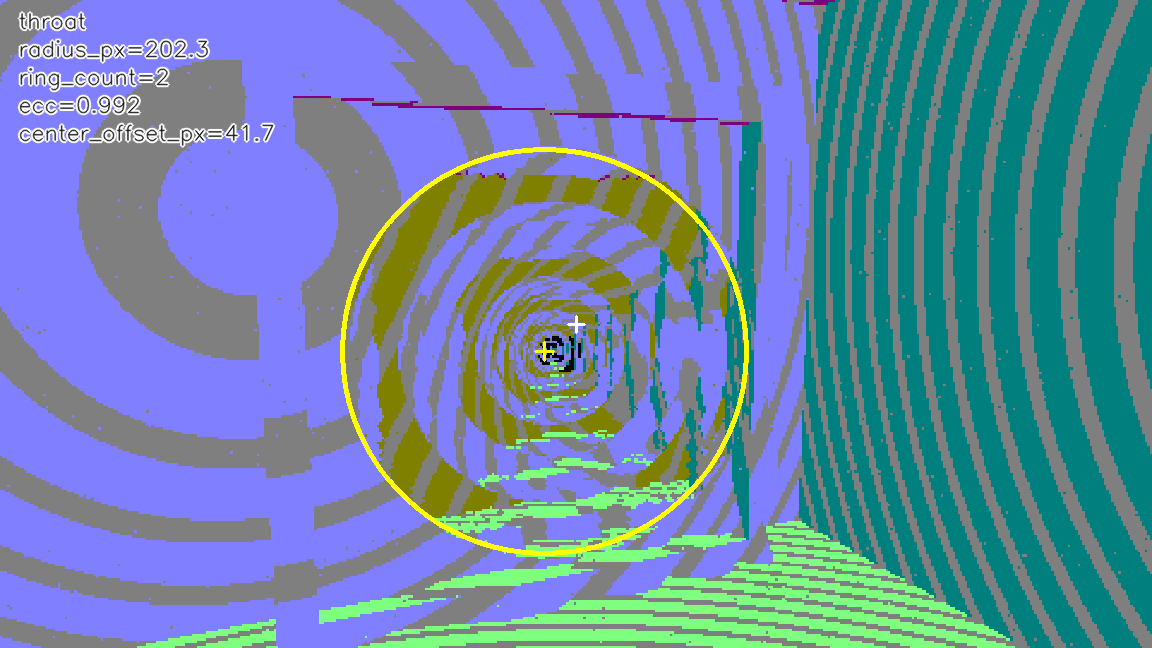
\includegraphics[width=0.48\textwidth]{../../paper_001_causal_observer_ladders/analysis/morphology/annotated/throat_annotated.png}
  \hfill
  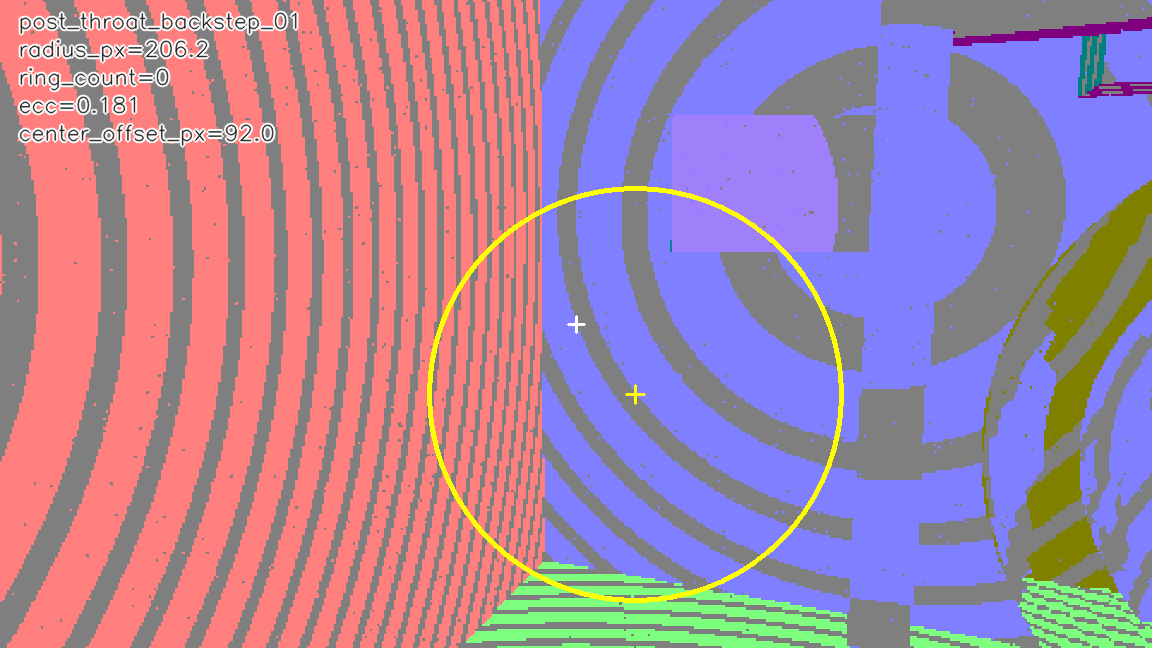
\includegraphics[width=0.48\textwidth]{../../paper_001_causal_observer_ladders/analysis/morphology/annotated/post_throat_backstep_01_annotated.png}
  \caption{Representative annotated morphology views for the throat checkpoint and the bridge checkpoint.}
\end{figure}

\begin{figure}[H]
  \centering
  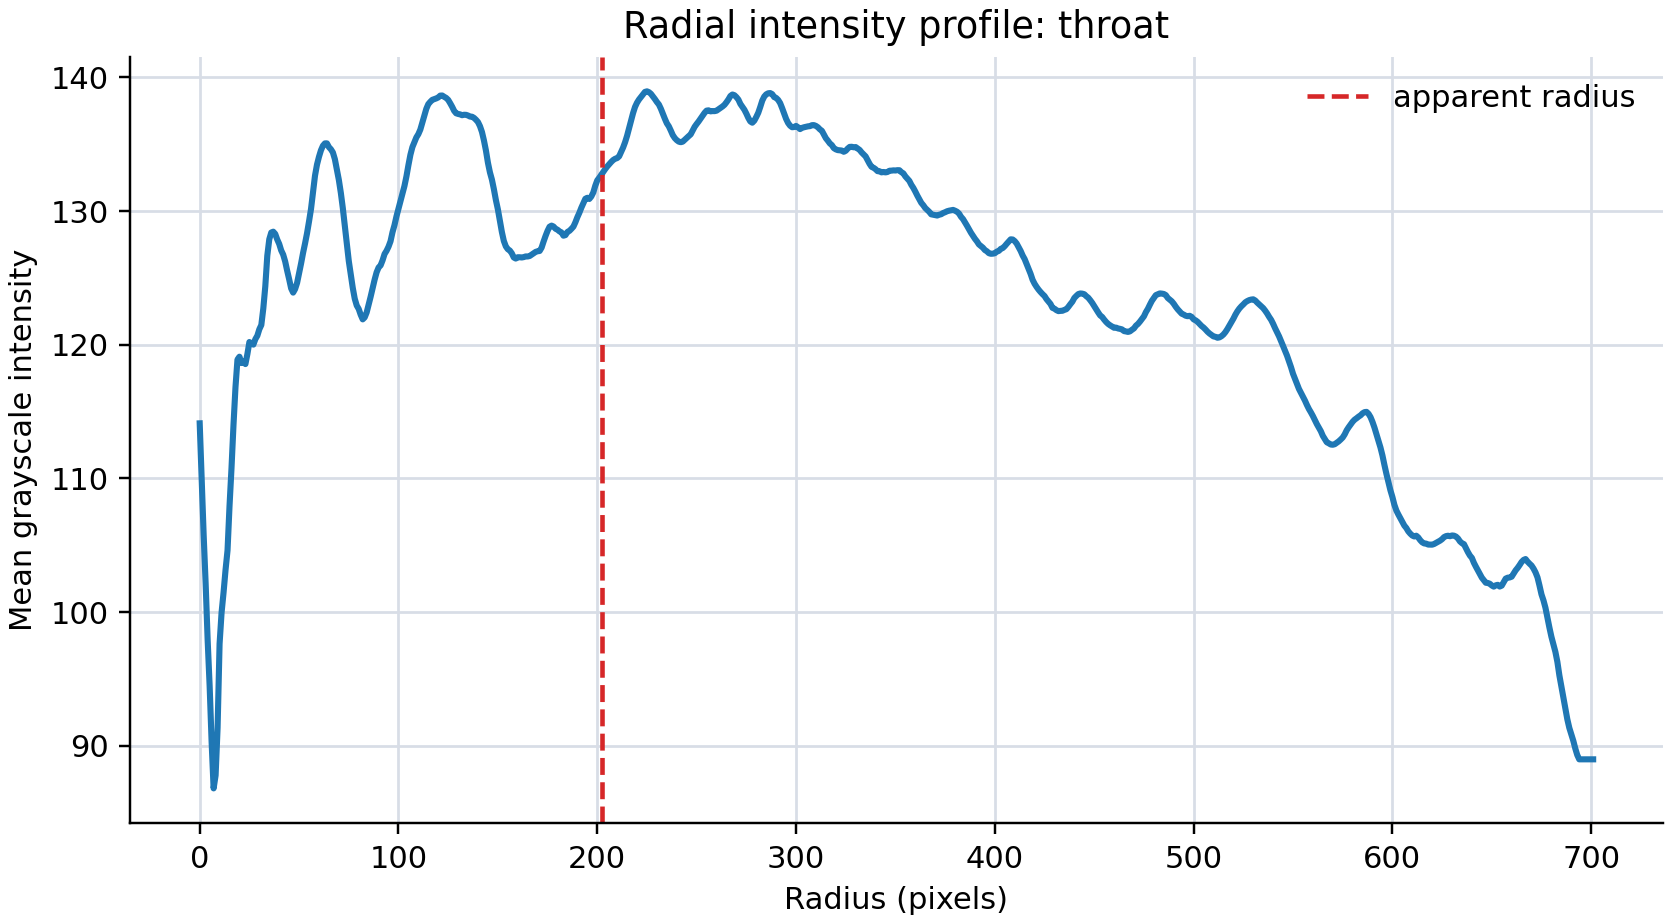
\includegraphics[width=0.48\textwidth]{../../paper_001_causal_observer_ladders/analysis/morphology/profiles/throat_radial_profile.png}
  \hfill
  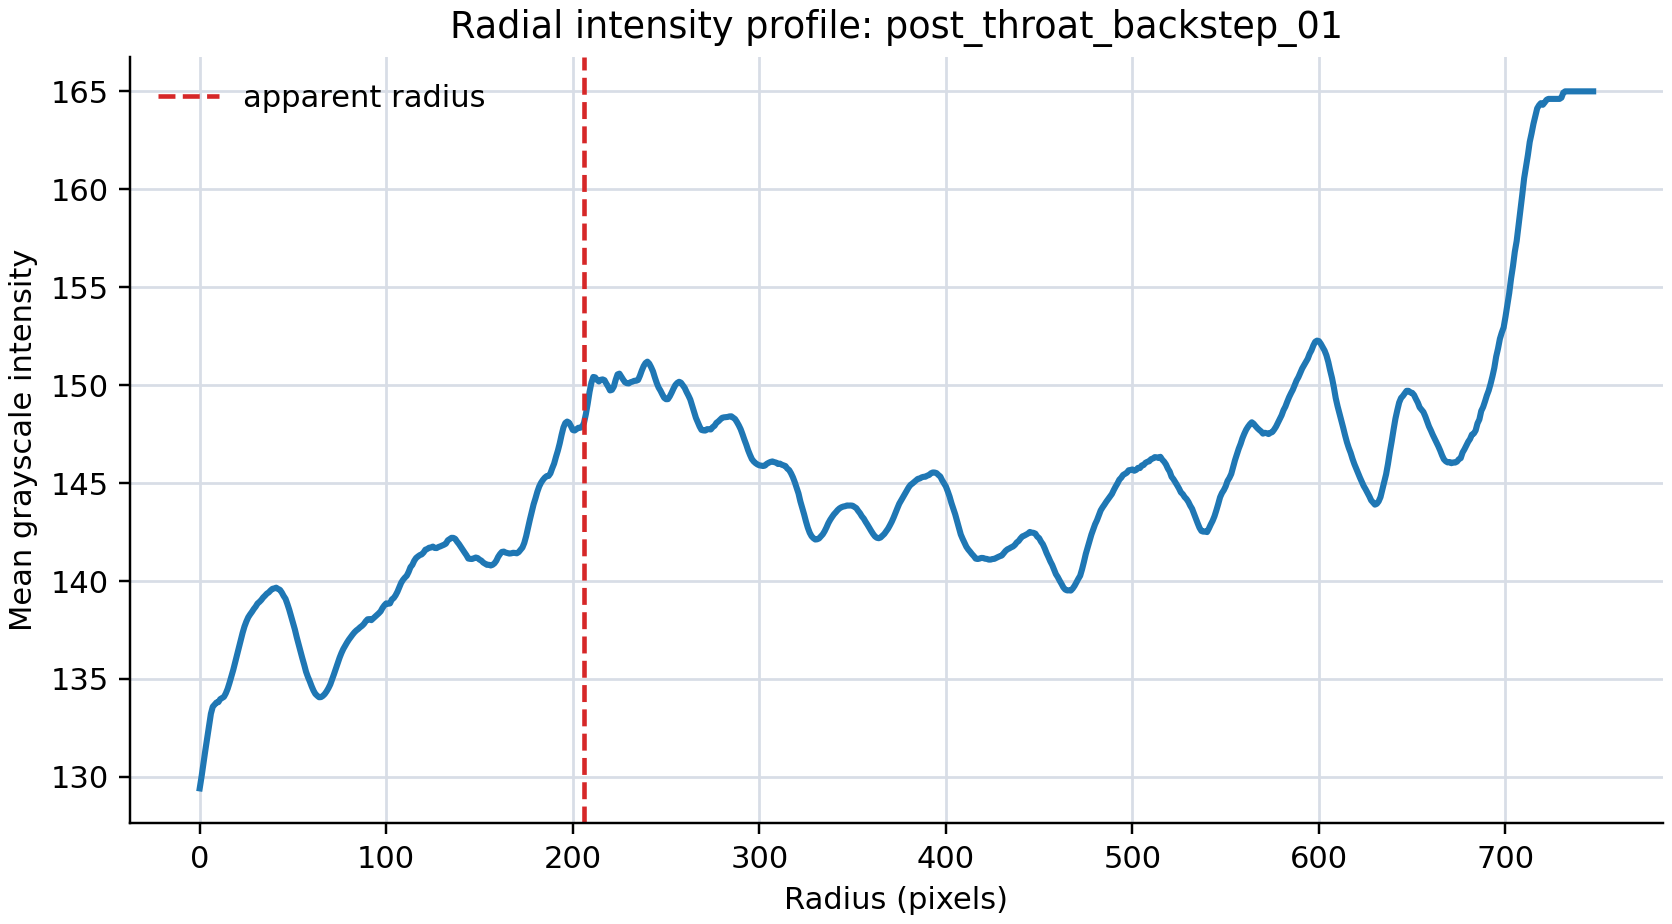
\includegraphics[width=0.48\textwidth]{../../paper_001_causal_observer_ladders/analysis/morphology/profiles/post_throat_backstep_01_radial_profile.png}
  \caption{Representative radial intensity profiles for the throat checkpoint and the bridge checkpoint.}
\end{figure}

\section{Reference Files}

\begin{itemize}
  \item \texttt{../../paper\_001\_causal\_observer\_ladders/figures/captions.md}
  \item \texttt{../../paper\_001\_causal\_observer\_ladders/clustering\_summary.md}
  \item \texttt{../../paper\_001\_causal\_observer\_ladders/analysis/regime\_clustering.md}
  \item \texttt{../../paper\_001\_causal\_observer\_ladders/analysis/bridge\_anomaly\_scoring.md}
  \item \texttt{../../paper\_001\_causal\_observer\_ladders/analysis/anomaly\_detection/summary.md}
  \item \texttt{../../paper\_001\_causal\_observer\_ladders/analysis/periodicity/summary.md}
  \item \texttt{../../paper\_001\_causal\_observer\_ladders/analysis/morphology/summary.md}
\end{itemize}

\end{document}
